\begin{frame}
\frametitle{bla}
\begin{tikzpicture}
  [level distance=1.2cm, 
   level 1/.style={sibling distance=4cm},
   level 2/.style={sibling distance=2cm},
   level 3/.style={sibling distance=1cm},
   level 4/.style={sibling distance=0.5cm},
   every node/.style={minimum size=6mm,inner sep=1pt,font=\tiny}]

  \node (root) {$\dots $}
    child {node (L1) {$\dots 0$} 
      child {node (L2a) {$\dots 00$} 
        child {node (L3a) {$\dots 000$}}
        child {node (L3b) {$\dots 100$}}
      }
      child {node (L2b) {$\dots 10$}
        child {node (L3c) {$\dots 010$}}
        child {node (L3d) {$\dots 110$}}
      }
    }
    child {node (R1) {$\dots 1$} 
      child {node (R2a) {$\dots 01$} 
        child {node (R3a) {$\dots 001$}}
        child {node (R3b) {$\dots 101$}}
      }
      child {node (R2b) {$\dots 11$}
        child {node (R3c) {$\dots 011$}}
        child  {node (R3d) {$\dots 111$}} % Leaf
      }
    };

  % Highlighting the path step by step
  \only<2->{\path[thick,red] (R3d) edge (R2b);} % Step 2: Highlight leaf to parent
  \only<3->{\path[thick,red] (R2b) edge (R1);}  % Step 3: Highlight next parent
  \only<4->{\path[thick,red] (R1) edge (root);} % Step 4: Highlight root connection

\end{tikzpicture}
\end{frame}

\begin{frame}
\frametitle{Highlighting a Path in the 2-adic Tree}

\begin{tikzpicture}
  [level distance=1cm, 
   level 1/.style={sibling distance=6cm},
   level 2/.style={sibling distance=3cm},
   level 3/.style={sibling distance=1.5cm},
   level 4/.style={sibling distance=0.75cm},
   level 5/.style={sibling distance=0.45cm},
   every node/.style={minimum size=6mm,inner sep=1pt,font=\tiny}]

  \node (root) {$\mydots$}
    child {node (L1) {$\mydots 0$} 
      child {node (L2a) {$\mydots 00$} 
        child {node (L3a) {$\mydots 000$}
          child {node (L4a) {$\mydots 0000$}}
          child {node (L4b) {$\mydots 1000$}}
        }
        child {node (L3b) {$\mydots 100$}
          child {node (L4c) {$\mydots 0100$}}
          child {node (L4d) {$\mydots 1100$}}
        }
      }
      child {node (L2b) {$\mydots 10$}
        child {node (L3c) {$\mydots 010$}
          child {node (L4e) {$\mydots 0010$}}
          child {node (L4f) {$\mydots 1010$}}
        }
        child {node (L3d) {$\mydots 110$}
          child {node (L4g) {$\mydots 0110$}}
          child {node (L4h) {$\mydots 1110$}}
        }
      }
    }
    child {node (R1) {$\mydots 1$} 
      child {node (R2a) {$\mydots 01$} 
        child {node (R3a) {$\mydots 001$}
          child {node (R4a) {$\mydots 0001$}}
          child {node (R4b) {$\mydots 1001$}}
        }
        child {node (R3b) {$\mydots 101$}
          child {node (R4c) {$\mydots 0101$}}
          child {node (R4d) {$\mydots 1101$}}
        }
      }
      child {node (R2b) {$\mydots 11$}
        child {node (R3c) {$\mydots 011$}
          child {node (R4e) {$\mydots 0011$}}
          child {node (R4f) {$\mydots 1011$}}
        }
        child {node (R3d) {$\mydots 111$} 
          child {node (R4g) {$\mydots 0111$}}
          child {node (R4h) {$\mydots 1111$}}
        }
      }
    };

  % Highlighting the path from the leaf ...1101 to the root
  \only<2->{\path[thick,red] (R4d) edge (R3b);} % Step 2: Highlight ...1101 -> ...101
  \only<3->{\path[thick,red] (R3b) edge (R2a);} % Step 3: Highlight ...101 -> ...01
  \only<4->{\path[thick,red] (R2a) edge (R1);}  % Step 4: Highlight ...01 -> ...1
  \only<5->{\path[thick,red] (R1) edge (root);} % Step 5: Highlight ...1 -> Root

\end{tikzpicture}

\end{frame}

\begin{frame}
\frametitle{2-adic Tree with Infinite Extension}

\begin{tikzpicture}
  [level distance=1.2cm, 
   level 1/.style={sibling distance=6cm},
   level 2/.style={sibling distance=3cm},
   level 3/.style={sibling distance=1.5cm},
   level 4/.style={sibling distance=0.75cm},
   level 5/.style={sibling distance=0.45cm},
   level 6/.style={sibling distance=0.15cm},
   every node/.style={minimum size=6mm,inner sep=1pt,font=\tiny}]

  % Tree Structure
  \node (root) {$\ZZ_2$}
    child {node (L1) {\mydots 0} 
      child {node (L2a) {\mydots 00} 
        child {node (L3a) {\mydots 000}
          child {node (L4a) {\mydots 0000}
            child [dashed] {node {0}}
          }
          child {node (L4b) {\mydots 1000}}
        }
        child {node (L3b) {\mydots 100}
          child {node (L4c) {\mydots 0100}}
          child {node (L4d) {\mydots 1100}}
        }
      }
      child {node (L2b) {\mydots 10}
        child {node (L3c) {\mydots 010}
          child {node (L4e) {\mydots 0010}
          child [dashed] {node {$34=100010^{(2)}$}}
          }
          child {node (L4f) {\mydots 1010}}
        }
        child {node (L3d) {\mydots 110}
          child {node (L4g) {\mydots 0110}
               child [dashed] {node {$38=100110^{(2)}$}}
          }
          child {node (L4h) {\mydots 1110}}
        }
      }
    }
    child {node (R1) {\mydots 1} 
      child {node (R2a) {\mydots 01} 
        child {node (R3a) {\mydots 001}
          child {node (R4a) {\mydots 0001}
            child [dashed] {node {$17=10001^{(2)}$}}
          }
          child {node (R4b) {\mydots 1001}}
        }
        child {node (R3b) {\mydots 101}
          child {node (R4c) {\mydots 0101}}
          child {node (R4d) {\mydots 1101}}
        }
      }
      child {node (R2b) {\mydots 11}
        child {node (R3c) {\mydots 011}
          child {node (R4e) {\mydots 0011}}
          child {node (R4f) {\mydots 1011}}
        }
        child {node (R3d) {\mydots 111} 
          child {node (R4g) {\mydots 0111}}
          child {node (R4h) {\mydots 1111}
            %child [dashed, gray, opacity=0.5] {node {\mydots 01111}}
            child [dashed] {node {$-1=\mydots 11111^{(2)}$}}
          }
        }
      }
    };

\end{tikzpicture}

\end{frame}
